%-----------------------------------LICENSE------------------------------------%
%   This file is part of tikz_figures.                                         %
%                                                                              %
%   tikz_figures is free software: you can redistribute it and/or              %
%   modify it it under the terms of the GNU General Public License as          %
%   published by the Free Software Foundation, either version 3 of the         %
%   License, or (at your option) any later version.                            %
%                                                                              %
%   tikz_figures is distributed in the hope that it will be useful,            %
%   but WITHOUT ANY WARRANTY; without even the implied warranty of             %
%   MERCHANTABILITY or FITNESS FOR A PARTICULAR PURPOSE.  See the              %
%   GNU General Public License for more details.                               %
%                                                                              %
%   You should have received a copy of the GNU General Public License along    %
%   with tikz_figures.  If not, see <https://www.gnu.org/licenses/>.           %
%------------------------------------------------------------------------------%

% Use the standalone class for displaying the tikz image on a small PDF.
\documentclass[crop, tikz]{standalone}

% Import the tikz and pgfplots packages to use for the drawing.
\usepackage{pgfplots, tikz}

% pgfplots package used.
\usepgfplotslibrary{groupplots}
\pgfplotsset{compat = 1.9}

% Begin the document.
\begin{document}

    % Draw the figure.
    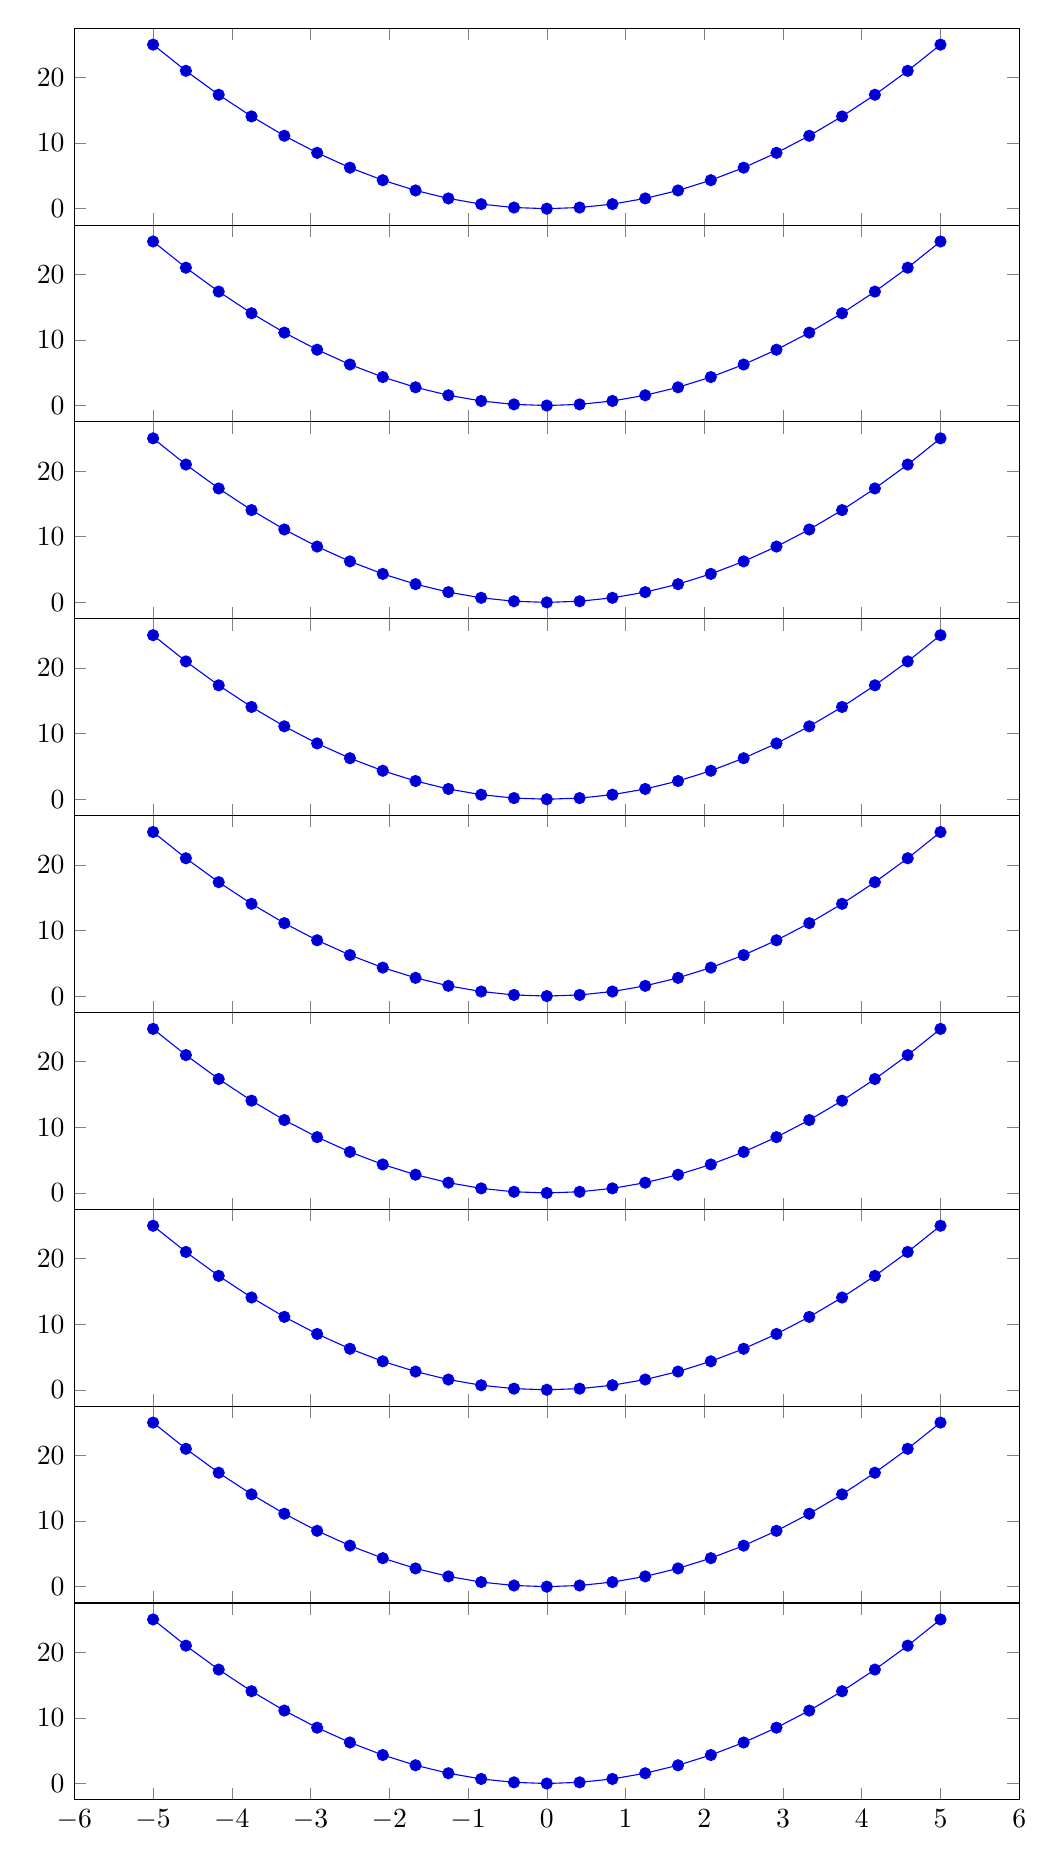
\begin{tikzpicture}

        % pgfplots can make several plots on one page using groupplots.
        \begin{groupplot}[
            group style = {%
                group name = geo1,
                group size = 1 by 9,
                vertical sep = 0pt,
                x descriptions at = edge bottom
            },
            width = 12cm,
            height = 2.5cm,
            scale only axis
        ]

            % Group plots example. Simple plot of x^2 done several times.
            \nextgroupplot\addplot {x^2};
            \nextgroupplot\addplot {x^2};
            \nextgroupplot\addplot {x^2};
            \nextgroupplot\addplot {x^2};
            \nextgroupplot\addplot {x^2};
            \nextgroupplot\addplot {x^2};
            \nextgroupplot\addplot {x^2}; 
            \nextgroupplot\addplot {x^2};
            \nextgroupplot\addplot {x^2};
        \end{groupplot}
    \end{tikzpicture}
\end{document}
